% Provenance (never printed): the production strand of ../economics_series.md (grade 8: factors of production, output
% per worker and per hour, capital per worker, better methods, productivity and living standards). Brief:
% sources/book1/BRIEFS.md, g8-01. Chart data: figdata/grade-8/01-production-and-productivity (PWT 11.0, 2023; Brenland
% firm census).
\chapter{Production and Productivity}\label{ch:g8:production-and-productivity}

\begin{openingchart}{Output per hour worked and income per person, 2023, one dot per
country (129 countries), in dollars of 2021, both on times-ten scales.}{Penn World Table
11.0: output-side real GDP divided by persons engaged times average hours; expenditure-side
real GDP divided by population}
\begin{tikzpicture}
\begin{loglogaxis}[omscatter, log ticks with fixed point, xmin=1, xmax=300, ymin=1000,
  ymax=200000, xtickten={0,...,3}, ytickten={3,...,6},
  xlabel={Output per hour worked (dollars of 2021, times-ten scale)},
  ylabel={Income per person (dollars of 2021)}]
\addplot table[x=oph, y=ipp] {figdata/grade-8/01-production-and-productivity/out/output_per_hour.csv};
\addplot[only marks, mark=*, mark size=1.6pt, omThm, nodes near coords, point meta=explicit symbolic,
  visualization depends on={value \thisrow{pos} \as \labelpos},
  every node near coord/.append style={font=\scriptsize, anchor=\labelpos, inner sep=2pt, text=black}]
  table[x=oph, y=ipp, meta=label] {figdata/grade-8/01-production-and-productivity/out/oph_labels.csv};
\end{loglogaxis}
\end{tikzpicture}
\end{openingchart}

% figdata: facts (NER_oph 2.4, IND_oph 8.1, CHN_oph 17.7, DEU_oph 82.5, USA_oph 83.5; NER_ipp 1900, IND_ipp 8700,
% DEU_ipp 59900, USA_ipp 74700; corr_log 0.97 is a rank correlation, not printed)
In 2023, an hour of work produced about $2.4$ dollars of goods and services in Niger, $8.1$
dollars in India, $17.7$ in China, $82.5$ in Germany and $83.5$ in the United States. The
dots lie almost on a line: where an hour of work produces more, people have higher \omterm{def:g7:households:income}{incomes}.
A person in Niger had an \omterm{def:g7:households:income}{income} of about $1\,900$ dollars in the year; a person in India
$8\,700$; in Germany $59\,900$; in the United States $74\,700$.

A country cannot consume, for long, more than it produces or can buy with what it produces.
This chapter asks what production needs, how to measure how much a worker produces, and why
some workers produce so much more than others.

\begin{recall}
\omterm{def:g6:living-standards:income-per-person}{Income per person} is a country's \omterm{def:g7:households:income}{income} divided by its population
(\cref{ch:g6:living-standards}). Dividing work into tasks raises \omterm{def:g7:specialisation:output-per-worker}{output per worker}
(\cref{ch:g7:specialisation}).
\end{recall}

\section{What production needs}

\begin{definition}[Factors of production]\label{def:g8:production-and-productivity:factors}
The \emph{factors of production}\index{factors of production} are the \omterm{def:g7:firms:input}{inputs} that an economy
uses to produce goods and services: \omterm{def:g8:production-and-productivity:labour}{labour}, capital, \omterm{def:g8:production-and-productivity:natural-resources}{natural resources} and \omterm{def:g8:production-and-productivity:technology}{technology}.
\end{definition}

\begin{definition}[Labour]\label{def:g8:production-and-productivity:labour}
\emph{Labour}\index{labour} is the work of people, measured in workers or in hours worked.
\end{definition}

\begin{definition}[Capital]\label{def:g8:production-and-productivity:capital}
\emph{Capital}\index{capital (physical)} (physical capital) is the stock of goods made by people
and used to produce other goods: tools, machines, vehicles, buildings, roads, networks.
\end{definition}

\begin{definition}[Natural resources]\label{def:g8:production-and-productivity:natural-resources}
\emph{Natural resources}\index{natural resources} are the \omterm{def:g7:firms:input}{inputs} given by nature: land, water,
minerals, oil and gas, forests and fish.
\end{definition}

\begin{definition}[Technology]\label{def:g8:production-and-productivity:technology}
\emph{Technology}\index{technology} is the knowledge of how to produce: methods, designs,
recipes, ways of organising work.
\end{definition}

\begin{omfigure}
\begin{tikzpicture}[econ, x=1cm, y=1cm,
  inp/.style={draw, rounded corners=2pt, fill=omDef!12, font=\scriptsize, minimum width=2.6cm,
    minimum height=0.7cm, align=center}]
  \node[inp] (l) at (0,1.65) {labour (hours of work)};
  \node[inp] (k) at (0,0.55) {capital (tools, machines)};
  \node[inp] (r) at (0,-0.55) {natural resources};
  \node[inp] (t) at (0,-1.65) {technology (methods)};
  \node[draw, very thick, fill=black!6, minimum width=2.4cm, minimum height=2.4cm, align=center,
    font=\small] (p) at (4.2,0) {production};
  \node[draw, rounded corners=2pt, fill=omMeth!15, font=\scriptsize, minimum width=2.4cm,
    minimum height=0.9cm, align=center] (o) at (8.2,0) {output: goods\\and services};
  \foreach \n in {l,k,r,t} \draw[-{Stealth}] (\n.east) -- (p.west);
  \draw[-{Stealth}, very thick] (p.east) -- (o.west);
\end{tikzpicture}

{\small Production combines the four factors. Each can be measured; the output is what the
economy makes in a year.}
\end{omfigure}

\section{Output per worker and per hour}

\begin{definition}[Labour productivity]\label{def:g8:production-and-productivity:labour-productivity}
\emph{Labour productivity}\index{labour productivity} is output divided by the \omterm{def:g8:production-and-productivity:labour}{labour} used to
produce it: \omterm{def:g7:specialisation:output-per-worker}{output per worker}, or output per hour worked.
\[
\text{output per hour} = \frac{\text{output}}{\text{number of workers} \times
\text{hours per worker}}.
\]
\end{definition}

\begin{example}
A Brenland workshop produces furniture worth $480\,000$ dalens in a year with 8 workers who
each work $1\,600$ hours. \omterm{def:g7:specialisation:output-per-worker}{Output per worker} is $480\,000 \div 8 = 60\,000$ dalens. Output per
hour is $480\,000 \div (8 \times 1\,600) = 480\,000 \div 12\,800 = 37.5$ dalens.
\end{example}

\begin{measure}[Output per hour]
The output of a country is its GDP (\cref{ch:g8:gdp}), converted into the same dollars for every
country at the \omterm{def:g7:money:price}{prices} of one year. Statisticians count the people who work, from \omterm{def:g8:production-and-productivity:labour}{labour} force
surveys and population censuses, and estimate the hours each works in a year. Hours are the hardest
part: they are measured carefully in rich countries and more roughly elsewhere. Output per hour is more
uncertain in poor countries, where many people work on their own farms or in small family
businesses.
\end{measure}

% figdata: facts (DEU_hours 1335, USA_hours 1789; DEU_opw 110.2, USA_opw 149.4)
Output per hour and \omterm{def:g7:specialisation:output-per-worker}{output per worker} can tell different stories. A worker in Germany worked
$1\,335$ hours in 2023, a worker in the United States $1\,789$. Per hour, the two produced
almost the same; per worker, the American produced $149.4$ thousand dollars, the German
$110.2$ thousand.

\begin{omfigure}
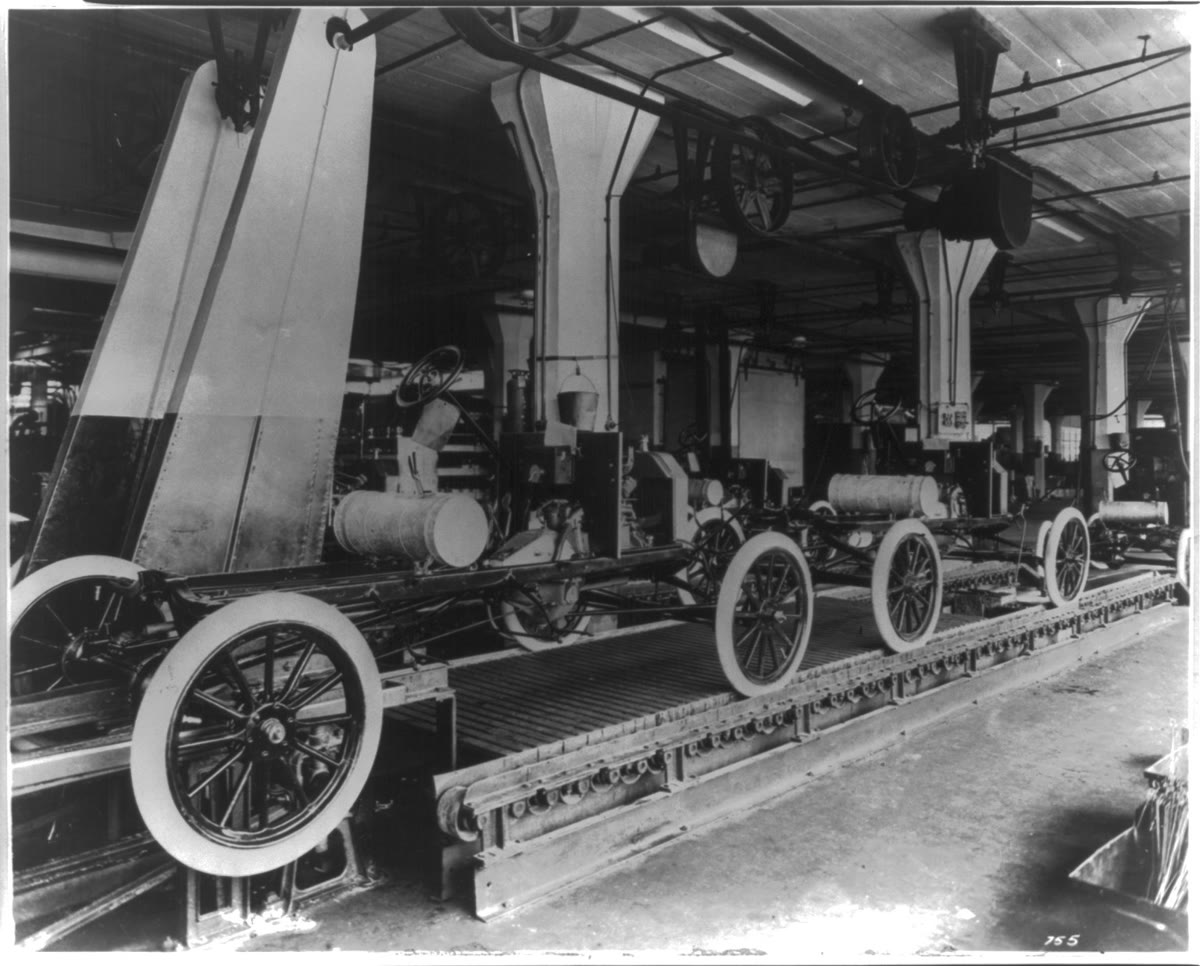
\includegraphics[width=0.58\linewidth]{images/book1/photos/g8-production-and-productivity-assembly-line-1913.jpg}

{\small A car assembly line in Michigan, United States, 1913. The chassis moves past workers
who each add a few parts: a new way of organising work, built around a new piece of capital,
the moving line.}
\end{omfigure}

\section{Capital per worker}

\begin{definition}[Capital per worker]\label{def:g8:production-and-productivity:capital-per-worker}
\emph{Capital per worker}\index{capital per worker} is the value of an economy's (or a \omterm{def:g7:firms:firm}{firm}'s)
capital divided by its number of workers.
\end{definition}

A farmer with a sickle cuts a small field in a day; with a harvester, the same farmer cuts many
times more. Workers with more and better machines produce more.

\begin{omfigure}
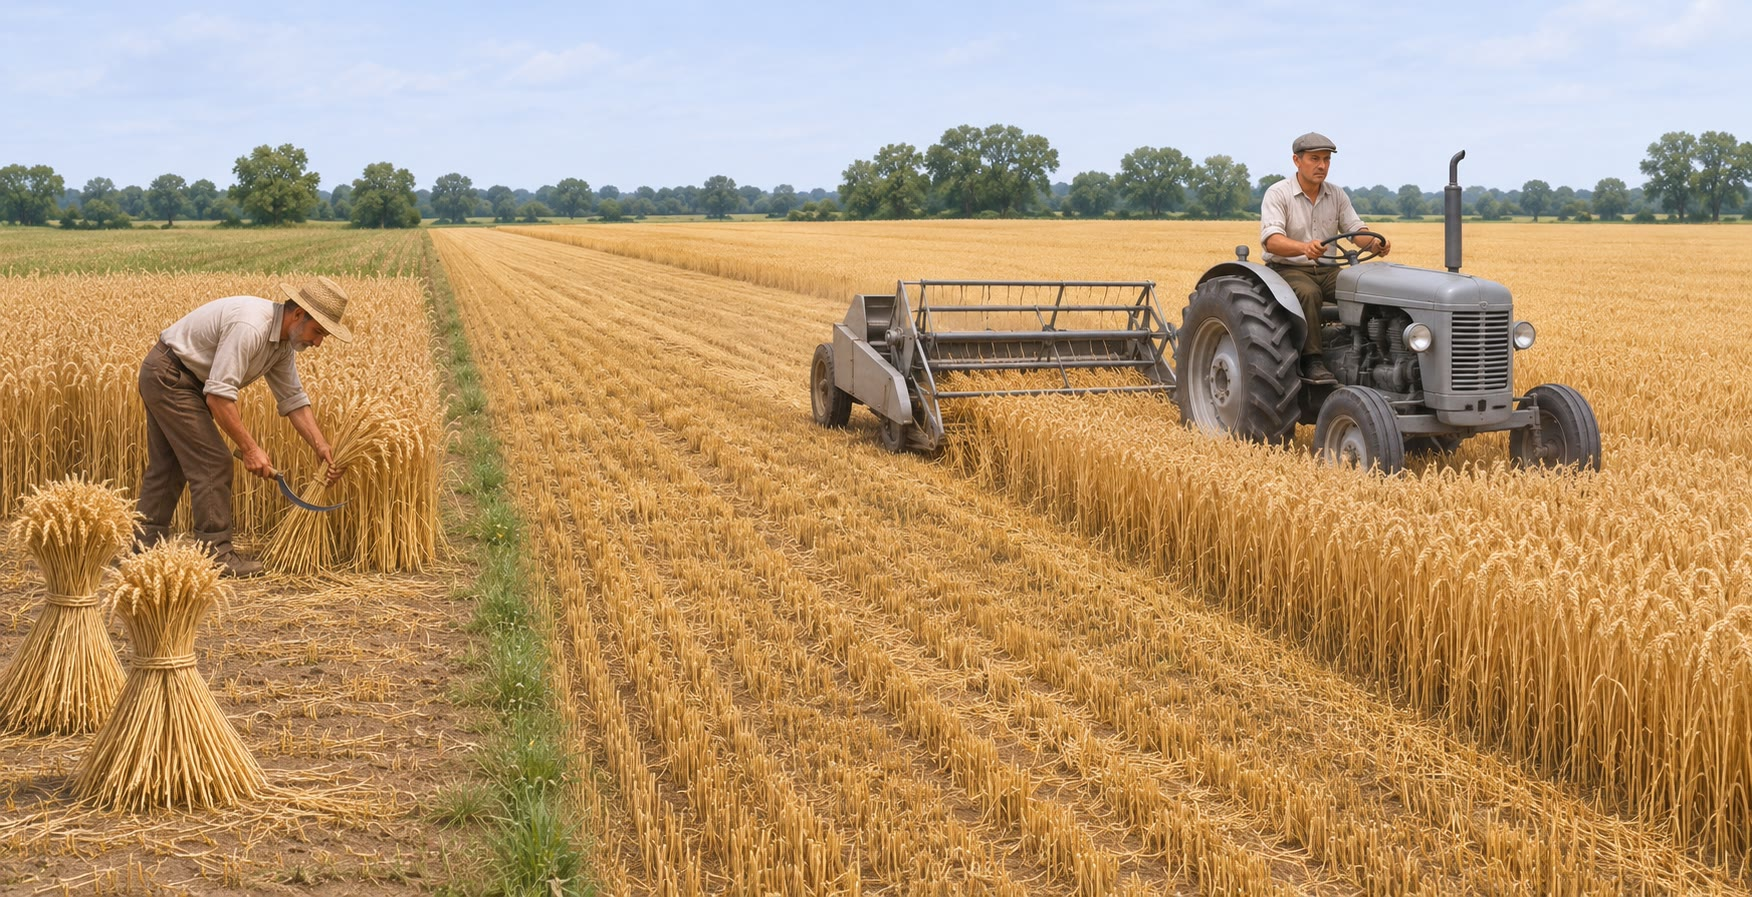
\includegraphics[width=0.52\linewidth]{images/book1/ai/g8-production-and-productivity-two-farmers.jpg}

{\small Two fields, the same wheat, the same sun: the difference is the capital each farmer works
with.}
\end{omfigure}

\begin{omchart}{Capital per worker and output per worker, 2023, one dot per country (173
countries), in thousands of dollars of 2021, both on times-ten scales.}{Penn World Table 11.0:
capital stock at constant national \omterm{def:g7:money:price}{prices} and output-side real GDP, each divided by persons
engaged}
\begin{tikzpicture}
\begin{loglogaxis}[omscatter, log ticks with fixed point, xmin=1, xmax=2000, ymin=0.5,
  ymax=500, xtickten={0,...,3}, ytickten={0,...,2},
  xlabel={Capital per worker (thousands of dollars, times-ten scale)},
  ylabel={Output per worker (thousands)}]
\addplot table[x=kpw, y=opw] {figdata/grade-8/01-production-and-productivity/out/capital_per_worker.csv};
\addplot[only marks, mark=*, mark size=1.6pt, omThm, nodes near coords, point meta=explicit symbolic,
  visualization depends on={value \thisrow{pos} \as \labelpos},
  every node near coord/.append style={font=\scriptsize, anchor=\labelpos, inner sep=2pt, text=black}]
  table[x=kpw, y=opw, meta=label] {figdata/grade-8/01-production-and-productivity/out/kpw_labels.csv};
\end{loglogaxis}
\end{tikzpicture}
\end{omchart}

% figdata: facts (NER_kpw 16.5, IND_kpw 76.8, KOR_kpw 523.1, USA_kpw 482.4; NER_opw 4.9, IND_opw 19.2, KOR_opw 102.4)
The dots again climb from the lower left to the upper right. A worker in Niger had $16.5$
thousand dollars of capital to work with and produced $4.9$ thousand dollars of output; a worker
in India, $76.8$ thousand and $19.2$ thousand; a worker in Korea, $523.1$ thousand and $102.4$
thousand. \omterm{def:g8:production-and-productivity:capital-per-worker}{Capital per worker} in Korea is about 32 times that in Niger, \omterm{def:g7:specialisation:output-per-worker}{output per worker} about 21
times. More capital goes with more output, but less than in proportion.

\begin{measure}[Measuring capital]
Nobody counts every machine and building in a country. Statisticians start from what is spent
each year on new machines, buildings and roads (investment), add it to the capital of the year
before, and subtract the part that wears out or becomes useless. Year after year, this running
total gives an estimate of the capital stock. It depends on guesses about how long each kind of
capital lasts.
\end{measure}

\section{Better methods}

More capital is not the whole story. In the scatter of capital and output, countries with the
same \omterm{def:g8:production-and-productivity:capital-per-worker}{capital per worker} produce different amounts: some use their machines with better methods,
better organisation and better-trained workers. A new method can raise output without any new
machine: rearranging a workshop so that parts flow from one task to the next, as on the assembly
line of the photograph, or using a seed that gives more grain per hectare. \omterm{def:g8:production-and-productivity:technology}{Technology}, the
knowledge of methods, spreads: once a method is known, other \omterm{def:g7:firms:firm}{firms} and countries can copy it.

\section{Why productivity sets the living standard}

\begin{model}{Productivity and living standards}
\assumes What a country consumes, it must produce, or buy with what it produces; its \omterm{def:g7:households:income}{income} is
the value of its output.
\predicts Countries with higher output per hour have higher \omterm{def:g7:households:income}{incomes} per person; countries with
more \omterm{def:g8:production-and-productivity:capital-per-worker}{capital per worker} produce more per hour.
\tested The opening chart (129 countries) and the chart of capital and output (173 countries).
\breaks Countries with oil and gas earn more than their workers' hours alone would give (Norway,
Qatar); in countries where a smaller share of people work, or where they work fewer hours, \omterm{def:g6:living-standards:income-per-person}{income
per person} is lower for the same output per hour; output can be recorded in a country but belong
to foreign owners (Ireland, \cref{ch:g8:gdp}).
\end{model}

% figdata: facts (NOR_oph 130.1, NOR_ipp 89100; QAT_oph 69.4, QAT_ipp 127100, QAT_hours 2435, QAT_part 69.1;
% DEU_part 54.5; IRL_oph 158.2)
\omterm{def:g6:living-standards:income-per-person}{Income per person} is output per hour, times the hours each worker works, times the share of
people who work. Qatar's output per hour, $69.4$ dollars, is below Germany's, yet its \omterm{def:g6:living-standards:income-per-person}{income per
person}, $127\,100$ dollars, is more than twice Germany's: its workers work $2\,435$ hours a year,
$69.1\,\%$ of its residents work, and it sells gas abroad. Ireland's output per hour, $158.2$ dollars, is the highest
in the chart; part of what is recorded there is the \omterm{def:g7:firms:profit}{profit} of foreign \omterm{def:g7:firms:firm}{firms}.

\section{Exercises}

\begin{exercise}[$\star$]\label{exo:g8:production-and-productivity:1}
Use the text. What was output per hour in India and in Germany in 2023? How many times larger
was it in Germany?
\end{exercise}

\begin{exercise}[$\star$]\label{exo:g8:production-and-productivity:2}
A bakery produces bread worth $360\,000$ dalens in a year with 6 workers. What is its \omterm{def:g7:specialisation:output-per-worker}{output per
worker}?
\end{exercise}

\begin{exercise}[$\star$]\label{exo:g8:production-and-productivity:3}
A factory produces $1\,800\,000$ dalens of goods in a year with 50 workers who each work $1\,600$
hours. Compute its output per hour.
\end{exercise}

\begin{exercise}[$\star$]\label{exo:g8:production-and-productivity:4}
Use the text. What was \omterm{def:g8:production-and-productivity:capital-per-worker}{capital per worker} in India and in Korea in 2023?
\end{exercise}

\begin{exercise}[$\star\star$]\label{exo:g8:production-and-productivity:5}
In countries A and B, each worker works $1\,700$ hours a year, and the same share of the
population works. Output per hour is 40 dollars in A and 60 dollars in B. Which has the higher
\omterm{def:g6:living-standards:income-per-person}{income per person}, and how many times higher?
\end{exercise}

\begin{exercise}[$\star\star$]\label{exo:g8:production-and-productivity:6}
In an invented workshop, \omterm{def:g7:specialisation:output-per-worker}{output per worker} depends on \omterm{def:g8:production-and-productivity:capital-per-worker}{capital per worker} as follows (thousands of
dalens):
\begin{center}
\begin{tabular}{lcccc}
\toprule
\omterm{def:g8:production-and-productivity:capital-per-worker}{Capital per worker} & 10 & 20 & 40 & 80 \\
\omterm{def:g7:specialisation:output-per-worker}{Output per worker} & 30 & 40 & 50 & 60 \\
\bottomrule
\end{tabular}
\end{center}
\omterm{def:g8:production-and-productivity:capital-per-worker}{Capital per worker} doubles from 20 to 40. Does \omterm{def:g7:specialisation:output-per-worker}{output per worker} double? By what percentage does
it rise?
\end{exercise}

\begin{exercise}[$\star\star$]\label{exo:g8:production-and-productivity:7}
A worker's hours fall from $1\,800$ to $1\,700$ a year, while output per hour rises from 50 to 54
dalens. Compute \omterm{def:g7:specialisation:output-per-worker}{output per worker} before and after. Did it rise or fall?
\end{exercise}

\begin{exercise}[$\star\star$]\label{exo:g8:production-and-productivity:8}
Use the opening chart and the last section. Name a country whose \omterm{def:g6:living-standards:income-per-person}{income per person} is far above
what its output per hour would give, and give two reasons.
\end{exercise}

\begin{exercise}[$\star\star$]\label{exo:g8:production-and-productivity:9}
Describe an observation that would contradict the model ``Productivity and \omterm{def:g6:living-standards:living-standard}{living standards}''.
\end{exercise}

\begin{exercise}[$\star\star\star$]\label{exo:g8:production-and-productivity:10}
A small economy has 600 farm workers who produce 20 dalens an hour and 400 factory workers who
produce 50 dalens an hour; all work the same hours. What is the average output per hour of all
workers?
\end{exercise}

\begin{exercise}[$\star\star\star$]\label{exo:g8:production-and-productivity:11}
In the economy of exercise 10, 100 farm workers move to factories, where they produce 50 dalens
an hour, like the other factory workers. What is the new average output per hour? Why did it rise
although no worker produces more in a given job?
\end{exercise}

\begin{exercise}[$\star\star\star$]\label{exo:g8:production-and-productivity:12}
The opening chart shows that output per hour and \omterm{def:g6:living-standards:income-per-person}{income per person} go together. Explain why the
chart alone cannot show which causes which, or whether a third thing causes both.
\end{exercise}

\section{Problem: Brenland's Factories}

\begin{problem}[{Weekend problem --- output per worker by sector in Brenland's firm census,
capital per worker, and 500 workers moving to manufacturing}]
\label{pb:g8:production-and-productivity:1}
% figdata: brenland_sectors (farming 51 firms 629 workers 65693 output 118157 capital; manufacturing 123, 1986,
% 188438, 312697; services 326, 5164, 361526, 326637)
Brenland's census of 2025 counts 500 \omterm{def:g7:firms:firm}{firms} (invented). The table gives, by sector, the number
of \omterm{def:g7:firms:firm}{firms}, their workers, their output and their capital, in thousands of dalens.
\begin{center}
\begin{tabular}{lrrrr}
\toprule
Sector & \omterm{def:g7:firms:firm}{Firms} & Workers & Output & \omterm{def:g8:production-and-productivity:capital}{Capital} \\
\midrule
Farming & 51 & 629 & 65\,693 & 118\,157 \\
Manufacturing & 123 & 1\,986 & 188\,438 & 312\,697 \\
Services & 326 & 5\,164 & 361\,526 & 326\,637 \\
\bottomrule
\end{tabular}
\end{center}

\medskip
\noindent\textbf{Part I --- Output per worker.}
\begin{enumerate}
  \item How many workers do the 500 \omterm{def:g7:firms:firm}{firms} employ in all?
  \item Compute \omterm{def:g7:specialisation:output-per-worker}{output per worker} in each sector, in thousands of dalens, to one decimal.
  \item Compute \omterm{def:g7:specialisation:output-per-worker}{output per worker} for all 500 \omterm{def:g7:firms:firm}{firms}.
  \item Which sector has the highest \omterm{def:g7:specialisation:output-per-worker}{output per worker}?
\end{enumerate}

\medskip
\noindent\textbf{Part II --- Capital per worker.}
\begin{enumerate}[resume]
  \item Compute \omterm{def:g8:production-and-productivity:capital-per-worker}{capital per worker} in each sector, to one decimal.
  \item Compute \omterm{def:g8:production-and-productivity:capital-per-worker}{capital per worker} for all 500 \omterm{def:g7:firms:firm}{firms}.
  \item Rank the sectors by \omterm{def:g8:production-and-productivity:capital-per-worker}{capital per worker}, and by \omterm{def:g7:specialisation:output-per-worker}{output per worker}. Is the order the same?
  \item How many times larger is \omterm{def:g8:production-and-productivity:capital-per-worker}{capital per worker} in farming than in services? And \omterm{def:g7:specialisation:output-per-worker}{output per
        worker}? Compare.
  \item Does the census show that farm workers work harder than service workers? Explain.
\end{enumerate}

\medskip
\noindent\textbf{Part III --- A move to manufacturing.} 500 service workers move to new
manufacturing \omterm{def:g7:firms:firm}{firms}. Each produces as much as the average manufacturing worker (use your rounded
answers to question 2); the service workers who stay produce as much as before.
\begin{enumerate}[resume]
  \item How many workers are now in manufacturing, and in services?
  \item Compute the new output of manufacturing and of services.
  \item Compute the new \omterm{def:g7:specialisation:output-per-worker}{output per worker} of all 500 \omterm{def:g7:firms:firm}{firms}, as a weighted average, to one decimal.
  \item What would the new manufacturing \omterm{def:g7:firms:firm}{firms} need, besides workers, for this to happen? Use
        part II.
\end{enumerate}
\end{problem}
